\section{Background}
In this section, we first introduce the brief background, including RDMA and virtualization. 

\subsection{RDMA}
As popular high-performance network in data-centers, RDMA has hardware protocol stack and zero copy technology. With RDMA, applications can bypass the kernel to read and write remote memory data, without the participation of remote CPU. 


In the workflow of RDMA, the control path and the data path are separated. As shown in Figure~\ref{fig:rdma-feat}, in the control path, the application creates QP(Queue Pair), CQ (Completed Queue), registers MR (Memory Region) and other RDMA resources, and caches the meta-data to RNIC, such as queue ID, MR key, page tables; In the data path, the application can "press"  the DoorBell register to notify RNIC, then RNIC will read the work request in the QP, read/write the contents of the local/remote MR, and put the completed notifications into the CQ. The data transmission is executed in zero-copy manner and without the CPU. And the application can poll the CQ to get the notifications. Compared control path, data path bypasses the kernel to avoid context switch.

RDMA can be implemented in different ways, for example, InfiniBand, Roce, and iWARP. However, Verbs is the general interface for applications. Verbs~\cite{verbs} is the basic interface for applications to utilize RDMA. It is similar as socket for traditional network applications. The control verbs include ibv\_create\_qp, ibv\_reg\_mr and so on; the data verbs include ibv\_post\_send and ibv\_post\_recv. 


\begin{figure}[!ht]
\centering
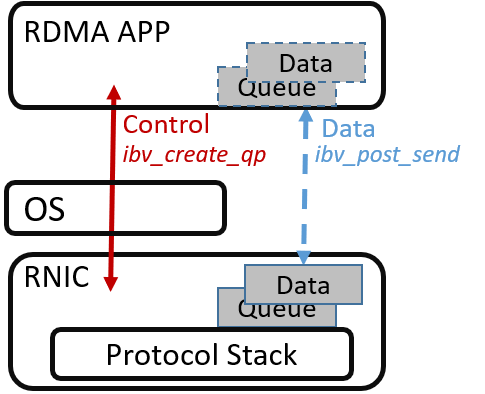
\includegraphics[width=0.8\linewidth]{images/rdma-feat.png}
\caption{Host RDMA Architecture: the control path and data path are separated}
\label{fig:rdma-feat}
\end{figure}


\subsection{Cloud and Virtualization}
Cloud is popular for its efficiency and elasticity, and virtualization is the basic for clouds. Nowadays, VMs and containers are both common virtual instances in clouds. VMs need emulate whole virtual hardware environments for guest operation system with hypervisor (kernel-space). So, applications in VMs is isolated by guest OS with more security but higher overhead. Containers are shared with the host OS but with run-time isolation. So, containers have low overhead and fast boot-up time.

For software virtualization of I/O devices, there are two main choices for where to emulate the device: kernel-space and user-space. In kernel-space, the codes of device emulation are inserted into hypervisor or host kernel. Compared to kernel-space, there are three advantages for user-space: first, the attack surface is limited for user-space with minimal inserted code into kernel/hypervisor; second, management development is flexible in user-space; third, the inserted codes are often dependent on kernel APIs (e.g. OS architecture, device driver). For example, vhost-net~\cite{vhost-net} is the kernel-space network device and vhost-user-net~\cite{vhost-user-net} has user-mode virtual device. 


